%%% machine_learning_p1.tex
%%%
%%% This LaTeX source document can be used as the basis for your technical
%%% paper or abstract. Intentionally stripped of annotation, the parameters
%%% and commands should be adjusted for your particular paper - title, 
%%% author, article DOI, etc.
%%% The accompanying ``template.annotated.tex'' provides copious annotation
%%% for the commands and parameters found in the source document. (The code
%%% is identical in ``template.tex'' and ``template.annotated.tex.'')

\documentclass[annual]{acmsiggraph}

\TOGonlineid{45678}
\TOGvolume{0}
\TOGnumber{0}
\TOGarticleDOI{1111111.2222222}
\TOGprojectURL{}
\TOGvideoURL{}
\TOGdataURL{}
\TOGcodeURL{}

\title{Supervised Learning Analysis and Report}

\author{Daniel A. Castro (dcastro9@gatech.edu) \\ CS-4641 - Machine Learning}
\pdfauthor{Daniel A. Castro}

\keywords{machine learning, cs4641, supervised learning}

\begin{document}

\maketitle

\section{Introduction of Datasets}

	In this report I am going to analyze two data sets over five different
types of supervised learning algorithms. These are the algorithms:
\begin{itemize}
\item Decision trees with pruning (Trees - J48)
\item Neural Networks (Functions - Multilayer Perceptron)
\item Boosting (Meta - AdaBoostM1)
\item Support Vector Machines (Functions - SMO)
\item k-nearest Neighbors (Lazy - IBk)
\end{itemize}

All of the algorithms are run through the Weka Explorer \cite{Hall_weka:2010}. The 
specifics for which algorithms were used within Weka are shown in parenthesis in 
the itemized list above.

The first dataset was obtained from~\cite{Frank+Asuncion:2010} and is titled the
Breast Cancer Wisconsin (Diagnostic) dataset. It containes 569 instances, and 31
different attributes. It was preprocessed to remove an arbitrary ID that each
instance contained, and converted to an arff file to simplify the processing in
the Weka Explorer. Of the 569 instances, it contains 357 benign samples, and 212
malignant samples.

The reason this dataset is interesting is because of its applicability in the
medical field. This dataset focuses on the classification problem for a breast
mass. It is of personal interest to me due to a personal passion to solve medical
problems through the use of modern-day technology. Further, it is of interest to
the machine learning algorithms because it requires very high levels of accuracy
in order to be useful to the community. Lastly, I found it relatively interesting
that there was a significant disparity between the false positives for the malignant
and benign categories. This could be attributed to a lack of completeness in the
data, given that there are significantly more benign samples in the dataset. The
high levels of accuracy that this dataset obtain indicate the potential for machine
learning to be able to tackle other diagnostic problems, eventually leading to a
more automated medical industry.

The second dataset was obtained from~\cite{Frank+Asuncion:2010} and is titled the 
One-hundred plant species leaves, by~\cite{Mallah:2013}. It contains 1600 instances, 64 different 
attributes, divided into three groups, for shape, margin, and texture. 
In this specific case, I decided to lower the complexity of the problem 
and only focus on the 64 texture attributes. The original dataset was much larger 
(192 attributes) and had a total of 4800 instances. The main motivation behind this
is to simply lower the complexity of the problem, given that there are only 16
instances available per class, and a total of 100 classes.

The reason this dataset is interesting is due to the complexity of the classification
problem. This dataset contains 100 separate classes, and each class has to train on
16 highly dimensional instances. Although some classes may be easily distinguishable,
I believe it is an ideal classification candidate to demonstrate the variance on the
parameters of each algorithm when dealing with binary classification vs the classification
of 100 classes.

\section{Methodology}

Our process for this experiment was to perform training and 10-fold cross validation
testing for each of the datasets on each of the supervised learning algorithms. In
each of these tests, I performed a number of iterations prior to obtaining a general
range of parameters in which the algorithm performs its best on the dataset. These
iterations will be graphed as I cover each of the datasets, in order to understand
broadly what varies between the algorithms for a highly dimensional classification
problem and contrast that with the parameters for binary classification. All of the
algorithms were run through Weka interface in order to obtain the results.

\section{Analysis of Wisconsin Dataset}

\subsection{Introduction}

The Wisconsin Dataset is a binary classification problem for breast masses which fall
into the benign or malignant category. The attributes for each category were based off
of measurements obtained from the mass, with the assumption that the size of the mass
was correlated to its classification.

The Wisconsin Dataset produced accurate results close to the 100 percentile. However,
after cross-validation for all of the tests, the results performed slightly worse. It
is important to note that every algorithm consistently obtained a much higher true
positive for the Benign mass classification than it did for the Malignant classification.
In fact, some algorithms even achieved a perfect classification after a 10-fold cross
validation, which was outstanding. However, this means that the malignant classification
suffered from false positives, which is not a desirable outcome given that the dataset
is part of an ongoing attempt to diagnose human conditions earlier in order to improve
treatment prior to symptoms worsening.

The false positives obtained for the malignant classification can most likely be attributed
to the lack of sufficient data for training. There was a significant amount more instances
for the benign classification than there were for the malignant classification, which would
explain why across each algorithm, the performance for malignant accuracy was worse.

\subsection{Data Analysis}

In this section I will break down the process that I took for each of the supervised learning
approaches. Overall, as shown by Table~\ref{tb:avgtimed1}, none of the algorithms took an excessive
amount of time to run for training or testing. The worst example was with boosting, where the
algorithm's were increasing linearly in training time due to the increase in number of iterations.

Further, I obtained decent results for accuracy shown by Table~\ref{tb:bestaccd1}, with boosting successfully 
obtaining the best test accuracy through 10-fold cross validation. For training, both boosting and 
kNN obtained a perfect score. 

\begin{table}
    \begin{tabular}{|c|c|c|} \hline
        Algorithm & Average Train Time & Average Test Time  \\ \hline
        Decision Trees & 0.100s & 0.020s \\
        Neural Networks & 0.021s & 3.156s \\
        Boosting & 7.100s & 0.030s \\
        SVMs & 0.152s & 0.030s \\
        k-Nearest Neighbors  & 0.01s & 0.172s \\
	\hline \end{tabular}
	\caption {Comparison of Algorithm Runtime} \label{tab:avgtimed1title}
	\label{tb:avgtimed1}
\end{table}

\begin{table}
    \begin{tabular}{|c|c|c|}
	\hline
        Algorithm           & Best Train Accuracy & Best Test Accuracy   \\ \hline
        Decision Trees      & 99.120\%             & 93.490\%            \\ 
        Neural Networks     & 99.470\%             & 97.890\%            \\ 
        Boosting            & 100.0\%              & 98.410\%            \\ 
        SVMs                & 98.240\%             & 98.067\%            \\ 
        k-Nearest Neighbors & 100.0\%              & 97.715\%            \\
	\hline \end{tabular}
	\caption {Comparison of Algorithm Performance} \label{tab:bestaccd1title}
	\label{tb:bestaccd1}
\end{table}

It is definitely important to highlight the high level of the accuracy that this
dataset achieves. I conclude that the dataset performs outstandingly well because
of the simplicity of the problem. Despite a somewhat average number of instances for
binary classification, the algorithms excel at solving the problem and achieving
impressive rates of accuracy. However, none of the algorithms reach a perfect test
accuracy rate after a 10-fold cross validation. I firmly believe that this is in part
due to random error which occurred in the data collection of the dataset, and also
in part due to the small number of instances. The reason which I believe it is due
to random error is because of the similarity in number of errors which every supervised
learning approach had. There was on average 2-6 instances of malignant false positives, 
and about 10-12 instances of benign false positives. which would suggest that the 
lower number of benign instances are due to the lack of data.

\subsubsection{Decision Trees}

\begin{figure}[ht]
  \centering
  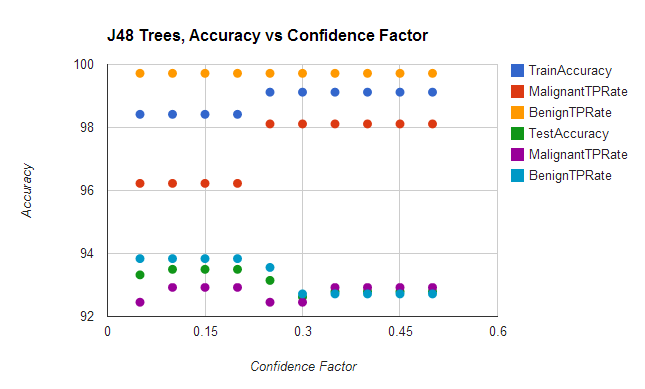
\includegraphics[width=3.5in]{charts/chart_1_j48_d1.png}
  \caption{This graph demonstrates the little effect that the confidence factor had on the dataset.}
  \label{fig:j48d1}
\end{figure}

For decision trees, I focused on using the J48 algorithm with error pruning, and then proceeded
to alter the confidence factor in order to see the potential changes in accuracy. As may be seen
in Figure ~\ref{fig:j48d1}, the benign true positive significantly outperformed the malignant true positive.
However, the malignant classification was much more strongly affected by altering the confidence
factor. In this sense, there is an interesting characteristic to learn from the data. At
approximately 0.25 confidence interval, there is a significant jump in accuracy for the benign classification
in training. This is most likely attributed to the classification attributes of the data set. Further, I see
how the testing results are less accurate in their classification, due to the rigor of a 10-fold test.

Lastly, the wall clock time for J48 trees in training was 0.1s and 0.02s in testing. The speeds
are simply due to the fact that this dataset only had 600 instances, and was a binary classification
problem.

\subsubsection{Neural Networks}

\begin{figure}[ht]
  \centering
  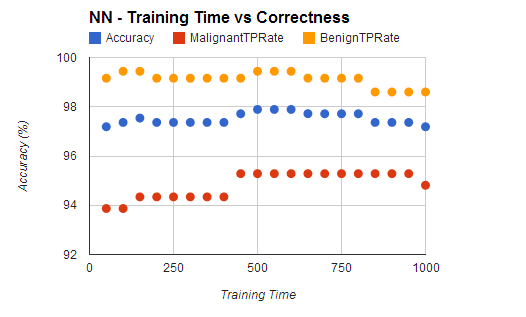
\includegraphics[width=3.5in]{charts/chart_2_nn_d1.png}
  \caption{Here I analyze the training time in order to understand if it has any effect on the accuracy.}
  \label{fig:nn3d1}
\end{figure}

Neural networks were sub-optimal in clock testing time at an average of 3.156s, but the algorithm
was incredibly fast in training, at 0.021s. I altered the learning rate of the network to 27 separate
values in an attempt to find the highest testing accuracy. I found this to be at a confidence interval
of 0.03. I also altered the training time parameter as can be seen in Figure~\ref{fig:nn3d1}, to obtain
that the best training time (best in the sense of obtaining the highest level of accuracy) was 500 epochs. 

The highest accuracy I was able to obtain in neural networks a 99.47\%, with zero malignant false positives,
and 3 benign false positives, at a learning rate of 0.95. Figure ~\ref{fig:nn1d1} demonstrates how this learning
rate was one of the many different tests which obtained very similar levels of accuracy. The training results
follow a vague direction but there does not seem to be a significant trend in its data. However, the testing data
seems to eliminate the random error in the results and demonstrate a more clear data (Figure ~\ref{fig:nn2d1}).

\begin{figure}[ht]
  \centering
  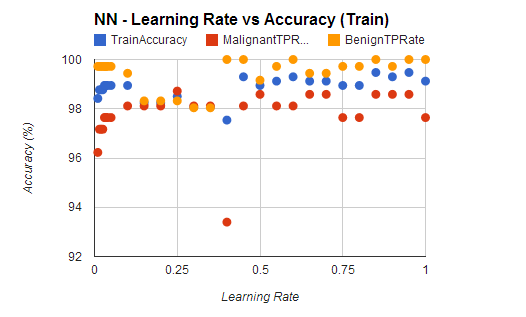
\includegraphics[width=3.5in]{charts/chart_3_nn_d1.png}
  \caption{The training for neural networks with the benign and malignant true positive rates. }
  \label{fig:nn1d1}
\end{figure}

However, in testing, the results demonstrated that a learning rate of 0.95 was not the optimal solution. In fact,
the best learning rate (in the sense of performance) was 0.03, obtaining an accuracy of 97.89\% with 2 malignant
false positives and 10 benign false positives. As stated earlier, the best explanation for the disparity in the number
of false positives for each class is the disparity in the number of instances to train on for each.

\begin{figure}[ht]
  \centering
  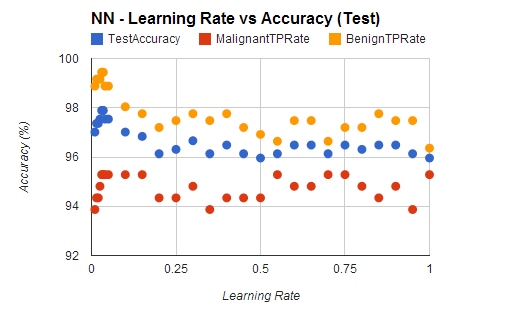
\includegraphics[width=3.5in]{charts/chart_1_nn_d1.png}
  \caption{The testing results for neural networks, with benign and malignant true positive rates. }
  \label{fig:nn2d1}
\end{figure}

Overall, the results for neural networks received one of the highest accuracy but ranked very poorly in its
testing time.

\subsubsection{Boosting}

Boosting performed accurately but took a significant amount of average train time. This average is skewed however,
since we ran the results until 2000 iterations which skew the average. For training, by 100 iterations, boosting
obtained 100\% accuracy at only 0.86s. The training and testing were all performed using the DecisionStump algorithm.

\begin{figure}[ht]
  \centering
  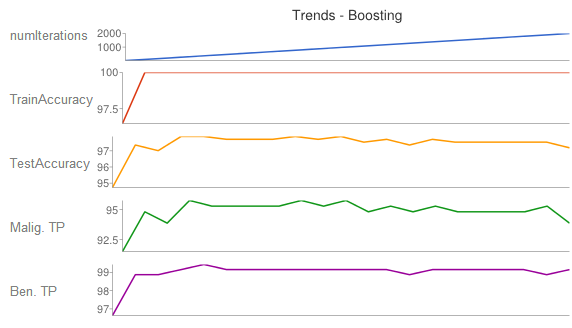
\includegraphics[width=3.5in]{charts/chart_1_boost_d1.png}
  \caption{As expected, boosting returns 100\% as can be seen in the train accuracy section. The interval for the number
  of iterations starts at 10, and then goes to 100, and from there rises in intervals of 100. This is why the graphs indicate
  a huge increment at the leftmost part of the graph. We tested the algorithm until 2000 iterations. The malignant and benign
  true positive results are after cross validation (testing), since training performed perfectly at 100+ iterations.}
  \label{fig:bb1d1}
\end{figure}

After performing the first boosting test, I decided to explore the accuracy differences due to the classifier. I tested the
different classifiers at 300 iterations. The results can be seen in Figure~\ref{fig:bb1d1}, where the LMT classifier
obtained the highest accuracy.

\begin{figure}[ht]
  \centering
  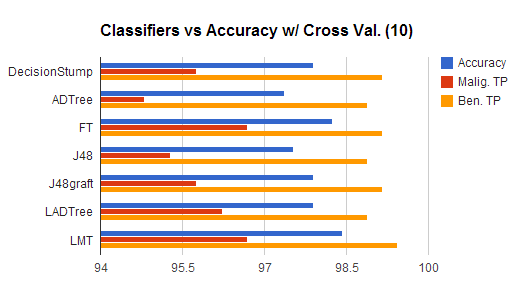
\includegraphics[width=3.5in]{charts/chart_2_boost_d1.png}
  \caption{The best performance for boosting on different classifiers was LMT.}
  \label{fig:bb2d1}
\end{figure}

It is interesting to notice in Figure ~\ref{fig:bb2d1} the disparity between the malignant and benign true positive rates. 
This gives a better sense of where the large number of error is coming from, which is the necessity for more instances of 
malignant tumors. To counter that however, if malignant tumors are less likely than benign tumors, it may not be wise to
normalize the data to obtain optimal performance.

\subsubsection{Support Vector Machines}

Support Vector Machines (SVMs) are very consistent in their accuracy for training in comparison to the accuracy for testing.
In training, SVMs obtain at best an accuracy of 98.24\%, while in testing the accuracy is at best a 98.06\%. This is in contrast
with other algorithms who perform rather poorly in testing because their training can easily reach 100\% due to their design 
(i.e. boosting) but when tested with 10-fold cross validation, they lose accuracy. We tested the complexity levels using a PolyKernel.

\begin{figure}[ht]
  \centering
  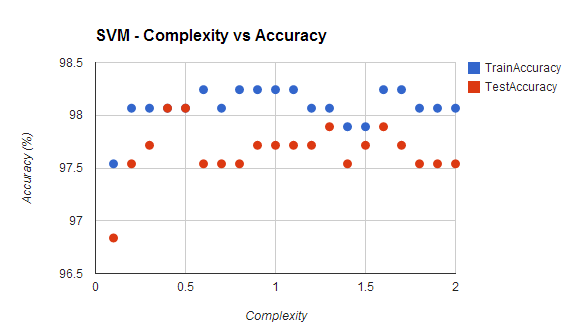
\includegraphics[width=3.5in]{charts/chart_1_svm_d1.png}
  \caption{Here it can be observed that accuracy did not seem to have a correlation with complexity.}
  \label{fig:svm1d1}
\end{figure}

Our first test compared the accuracy of SVMs due to the change in c, the complexity parameter. Figure ~\ref{fig:svm1d1} demonstrates
how incrementing the complexity did not have a significant effect on accuracy. However, there is an interesting phenomenon that can
be observed in the figure above. In some cases, like at a complexity of 0.4 or 0.5, the accuracy for training was identical to the accuracy for testing. This is a trait that was not observed in any of the previous algorithms. In fact, this complexity level 
obtained the best testing performance which is why we proceeded to use it to test a change in kernel.

\begin{figure}[ht]
  \centering
  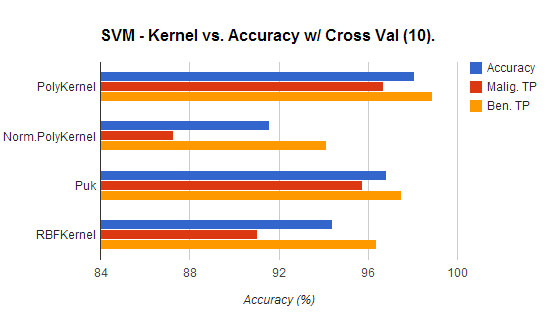
\includegraphics[width=3.5in]{charts/chart_2_svm_d1.png}
  \caption{This demonstrates the difference in performance for different kernels.}
  \label{fig:svm2d1}
\end{figure}

Alternating the kernel confirmed that the PolyKernel was the best kernel for this dataset. It obtained the best overall accuracy, and the
best malignant and benign true positive rates. The results are clearly demonstrated in Figure~\ref{fig:svm2d1}.

\subsubsection{K-Nearest Neighbors}

For k-nearest neighbors we used the iBk algorithm and altered the following parameters:
\begin{itemize}
\item Value of k
\item Distance Weighting
\item Mean Squared
\item Cross Validate when Picking K (hold one out)
\end{itemize}

First, we performed the study for the odd values of k from 1 to 25, and then chose arbitrary k's at 30, 35, 40, 50, and 100 to understand
the effect that k would have on performance. This study produced an interesting hypothesis - the malignant data instances were highly 
vulnerable to the increments in k values, whilst the benign instances remained constant in their accuracy even at k=100. These results
can be observed in ~\ref{fig:knn1d1} or ~\ref{fig:knn2d1}, where the malignant true positive trend is clearly dropping while the
benign trend remains nearly constant.

Our best results were at k=9 for overall accuracy, but k=15 obtained a higher benign true positive. This is particularly important
to note because it may be in the interest of the system you build to use different machine learning techniques to confirm or reject
your results and further prevent your error. For instance, if this system to test for tumors were to be implemented with kNN at
k=9, and your result was benign, a smart way of incrementing the confidence of your result would be to test the same result at k=15.

\begin{figure}[ht]
  \centering
  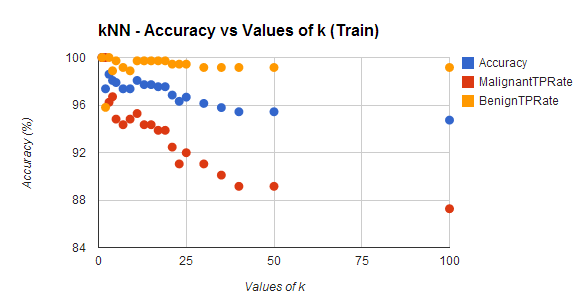
\includegraphics[width=3.5in]{charts/chart_2_knn_d1.png}
  \caption{Training for knn demonstrates a loss in performance for malignant TP rates.}
  \label{fig:knn2d1}
\end{figure}

\begin{figure}[ht]
  \centering
  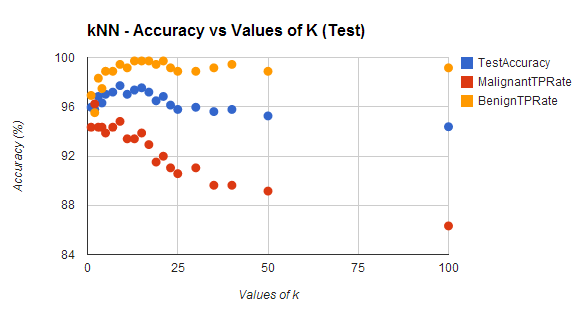
\includegraphics[width=3.5in]{charts/chart_1_knn_d1.png}
  \caption{Testing performed on different k parameters through 10-fold cross-validation.}
  \label{fig:knn1d1}
\end{figure}

We also conducted tests on distance weighting on select values of k which performed optimally (2, 7, 9, 13, 15, 17 and 21). In these
results, distance weighting and mean squared had no effect on improving the algorithm (it remained the same for all but k=2, in which 
it did worse, potentially because k=2 doesn't break ties). Further, I activated cross validation, wherein the algorithm will leave
a random k value out from choosing in order to perform a stronger test. For the values of k I previously stated, the algorithm did
not change its performance which demonstrates the strength in the relationship the attributes have to their own class. In this case,
2 was the only one which performed worse for obvious reasons (you are leaving one of your two k values out of the comparison).

\subsection{Performance Comparison}

In conclusion of the breast mass dataset, we obtained our best testing performance from boosting, with the LMT classifier at 300
iterations. Boosting at 300 iterations with an LMT classifier did not perform significantly different in training and testing time
which is why it supersecedes the other algorithms. 

\section{Analysis of Plant Species Dataset}

\subsection{Introduction}

The Plant Dataset is an incredibly complex dataset that strives to learn from
the characteristics of the leaves of plants. By learning from these using
supervised learning techniques from machine learning, one should be able to
categorize any unknown leaf as one of the leaves. The problem with the dataset
is that it is separated into three different sets of data, for the leaves shape,
the leaves texture, and the leaves margin. Each of these files contains 16
instances on each of the 100 different types of leaves, with 64 attributes per
instance. I decided to focus specifically on the texture of the leaves as my
classification, for the scope of this assignment.

All of the attributes are real values, and were all converted to arff files
for easy use with the weka interface. A lot of the testing results for the
Plant Dataset required a significant amount of analysis in order to obtain
results that were not incredibly poor. The biggest problem that this dataset
suffers from is its high complexity. When performing cross validation, the leaf
you are testing for may have very few number of leaves to test against. Given
that the original dataset only has 16 instances per class, in this sense cross
validation may fail due to the assumptions it makes about the data it is testing.

The results of the data for this part of this assignment are available upon request,
some of the outputs were upwards of 300MB in size, for which they were not attached
or shared (due to the magnitude of the file). They generally provided 100x100 charts
for false positives, but it was incredibly difficult to examine these results or
extract useful information from them. The dataset actually does come with black
and white images of the leaves which are interesting to look at in order to see
why some leaves could get confused with others.

\subsection{Data Analysis}

As we can see in Table~\ref{tb:avgtimed2}, neural networks and SVMs took a 
relatively large amount of time when compared with the other algorithms. Due to
the average time that the algorithm takes to compile, it is reasonable that
neural networks performs the best classification after a 10-fold cross validation.
However, boosting, which was relatively inexpensive (clock wise), performs better
than SVMs in testing (Table ~\ref{tb:bestaccd2}).

Overall, the algorithms performed surprisingly well for the complexity of the
data set, and for future work it would be intriguing to see if the use of more
data could improve the accuracy.

\begin{table}
    \begin{tabular}{|c|c|c|} \hline
        Algorithm & Average Train Time & Average Test Time  \\ \hline
        Decision Trees & 0.831s & 0.100s \\
        Neural Networks & 424.126s & 0.347s \\
        Boosting & 0.28s & 0.04s \\
        SVMs & 17.23s & 140.129s \\
        k-Nearest Neighbors  & 0.01s & 0.5s \\
  \hline \end{tabular}
  \caption {Comparison of Algorithm Runtime} \label{tab:avgtimed2title}
  \label{tb:avgtimed2}
\end{table}

\begin{table}
    \begin{tabular}{|c|c|c|}
  \hline
        Algorithm           & Best Train Accuracy & Best Test Accuracy   \\ \hline
        Decision Trees      & 90.494\%             & 52.53\%            \\ 
        Neural Networks     & 97.56\%             & 83.98\%            \\ 
        Boosting            & 100.0\%              & 82.55\%            \\ 
        SVMs                & 97.240\%             & 81.17\%            \\ 
        k-Nearest Neighbors & 100.0\%              & 80.11\%            \\
  \hline \end{tabular}
  \caption {Comparison of Algorithm Performance} \label{tab:bestaccd2title}
  \label{tb:bestaccd2}
\end{table}

\subsubsection{Decision Trees}

\begin{figure}[ht]
  \centering
  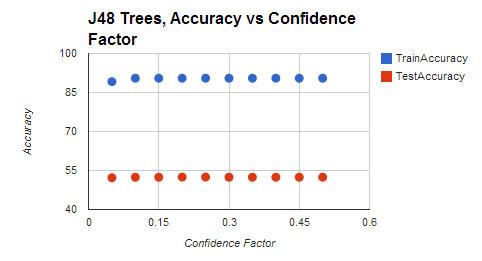
\includegraphics[width=3.5in]{charts/chart_1_j48_d2.PNG}
  \caption{Varying the confidence factor of the j48 algorithm.}
  \label{fig:j481d2}
\end{figure}

Decision trees had the worst test performance out of the five learning algorithms.
The trianing accuracy was actually relatively good but decision trees were particularly
vulnerable to losing percentages of the data in order to do cross-validation. They
suffered a nearly 40\% drop in accuracy, at a best of 52.53\%. It turns out that
because of the small number of instances, pruning actually hurts the classification,
with the best result (52.53\%) actually resulting from the unpruned test. The best
pruned result was close behind at 52.41\%.

In this experiment we altered the confidence factor from 0.05 to 0.50 with an
interval of 0.05. There was no significant change in the accuracy of the results. 

\subsubsection{Neural Networks}

\begin{figure}[ht]
  \centering
  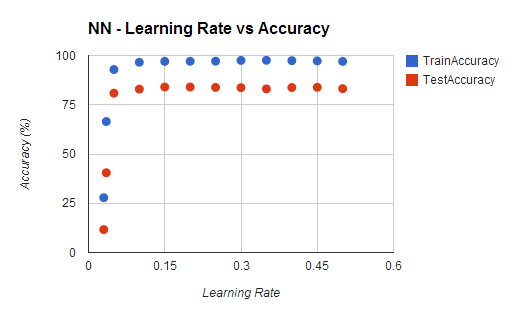
\includegraphics[width=3.5in]{charts/chart_1_nn_d2.PNG}
  \caption{The learning rate of neural networks did not have a significant
  effect after incrementing past a learning rate of 0.10.}
  \label{fig:nn1d2}
\end{figure}

Neural networks had the best performance on our learning algorithms. The learning
rate was placed at 0.03, 0.035, and then intervals of 0.05 from 0.05 to 0.5. The
main motivation behind testing at 0.03 and 0.035 was to compare against the parameters
that performed the best in our first dataset. Interestingly enough, the best
performing parameters obtained the worst results for the neural network dataset.
From this we can infer that for a highly complex classification with very few
instances per class, it is more convenient to have a greater learning rate.

\begin{figure}[ht]
  \centering
  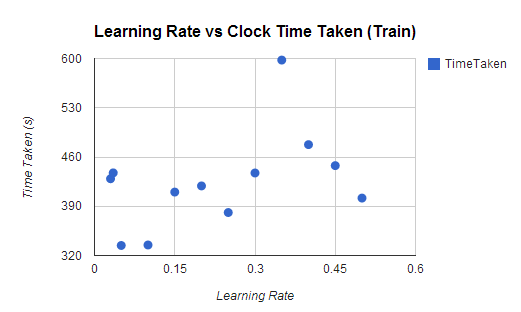
\includegraphics[width=3.5in]{charts/chart_2_nn_d2.PNG}
  \caption{We graphed the clock time against its learning rate and there
  seemed to be no correlation.}
  \label{fig:nn2d2}
\end{figure}

Lastly, we compared the learning rate to its clock time (Figure~\ref{fig:nn2d2}, 
in order to see if there was any significance, but there was no apparent 
correlation between greater learning rates and the time taken to train the 
neural network. This is logical, but also provides insight into how the learning 
rate can affect the complexity of building the neural network (assuming more 
complex neural networks take longer to build).

\subsubsection{Boosting}

Boosting presented incredible insight into the functioning of decision stumps.
The decision stump was simply unable to handle the complexity of the dataset.
The training dataset obtained an accuracy of 2\%, with a testing accuracy of
1.26\%. The poor results can be seen in Figure~\ref{fig:boost1d2}. However, after
diagnosing that the number of iterations for decision stump had no effect in 
changing the performance, I decided to test the algorithm using J48 as the classifier.

\begin{figure}[ht]
  \centering
  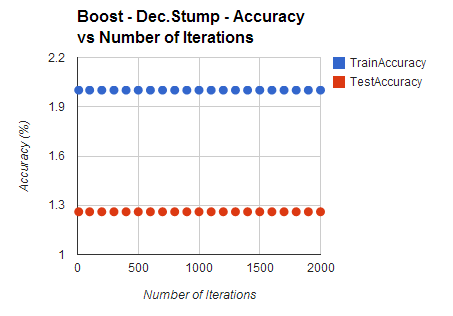
\includegraphics[width=3.5in]{charts/chart_1_boost_d2.PNG}
  \caption{The incredibly poor accuracy of using decision stump in the boosting
  algorithm.}
  \label{fig:boost1d2}
\end{figure}

In Figure~\ref{fig:boost2d2}, we see a much better performance with boosting,
using J48. We performed iterations from 10 to 100 in intervals of 10. After 50
intervals, the accuracy in the results seemed to approach a maximum of ~83\%.

In general, we observe that DecisionStump prefers simpler classifications, and
can perform only perform slightly better than chance (1/100 would be chance and
it's performing at 2/100).

\begin{figure}[ht]
  \centering
  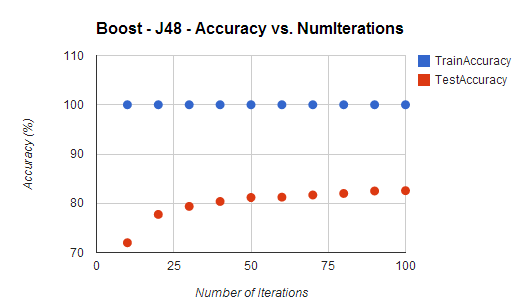
\includegraphics[width=3.5in]{charts/chart_2_boost_d2.PNG}
  \caption{The accuracy of training and testing by using J48.}
  \label{fig:boost2d2}
\end{figure}

\subsubsection{SVMs}

For SVMs, I focused on altering the complexity parameter from 0.1 to 2, with an
interval of 0.1. We used the PolyKernel as the kernel of the SVMs. It's very
intriguing to notice how after approximately 140 seconds the time that the
algorithm takes continues to increase while the accuracy stalls. 

\begin{figure}[ht]
  \centering
  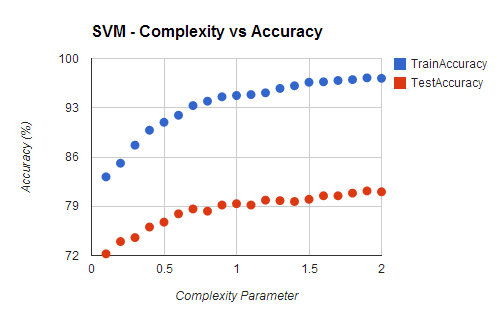
\includegraphics[width=3.5in]{charts/chart_1_svm_d2.PNG}
  \caption{Accuracy after a complexity of 1.5 stalls at approximately 97.24\% 
  for training, and 81.17\% for testing.}
  \label{fig:svm1d2}
\end{figure}

\begin{figure}[ht]
  \centering
  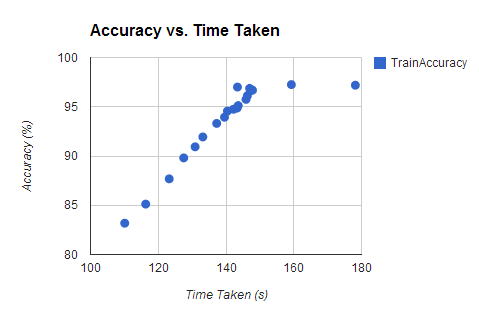
\includegraphics[width=3.5in]{charts/chart_2_svm_d2.PNG}
  \caption{Accuracy stalls after about 140 seconds of performance.}
  \label{fig:svm2d2}
\end{figure}

Overall, SVMs perform decently well but take too long to test. On average, an
SVM test took 140.129 seconds, in comparison to boosting which took 0.04 seconds,
and obtained better cross validation test accuracy.

\subsubsection{K-Nearest Neighbors}

In k-nearest neighbors, we obtained an ideal example of how using more neighbors
simply decreases the accuracy. It can specifically be explained by the number
of instances available per class. Once you attempt to train by a greater k, the
probability for you to get more errors increases significantly. This is further
extrapolated by using 10-fold cross validation, which explains the errors which 
you may see in Figure~\ref{fig:knn1d2}.

\begin{figure}[ht]
  \centering
  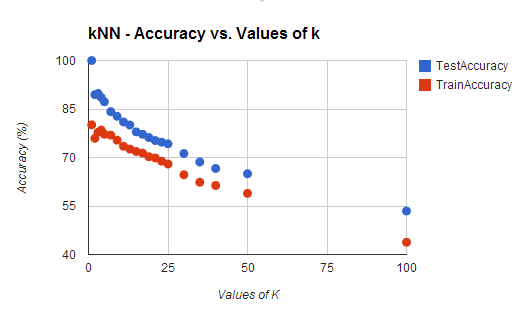
\includegraphics[width=3.5in]{charts/chart_1_knn_d2.PNG}
  \caption{**The labels are flipped in this diagram. Blue represents the training data,
  and red represents the testing data. The figure demonstrates the drop in performance as we increment k.}
  \label{fig:knn1d2}
\end{figure}

\subsection{Performance Comparison}

In training, boosting obtained the best performance at 100\%. However, for testing,
neural networks obtained better accuracy. It is also worth noting that decision
trees had the greatest disparity between training and testing because the algorithm
simply could not deal with the low number of instances per class and the complexity
of the classification problem.

\section{Results - General Comparison}
The best connection between the two datasets can be observed in neural networks,
where the parameters for best performance in the Breast Mass dataset were the
worst parameters for the neural network. Further, for the kNN experiment, we 
observed how k=9 and even k=15 performed decently well in the binary classification.
However, a k=9 or k=15 for the second dataset were terrible in relation to k=1. 
This is due to the complexity of both datasets, given that in binary classification,
it is a 50/50 problem at worse, whilst in the 100 class plant dataset, the performance
for breaking a tie or simply guessing is 1/100. Further, it is incredibly easier
to obtain ties in these situations because you could obtain unique number of classes
even at k=100. For boosting, it was better to observe performance with the number
of iterations to be below 100 for the larger dataset. It was simply not computationally
reasonable to perform boosting at large amounts for such a large dataset since we
had achieved a training of 100\% with an adequate runtime. For SVM's, the best complexity
level for the breast mass dataset was 0.4, and approximately 1.5 for the more complex
dataset. For both datasets, varying the confidence factor does not seem to have
an incredibly significant effect. 
\section{Conclusion}
After analyzing the results, it becomes rather evident that these algorithms
expose a lot more about the data than is originally presented. These supervised
learning techniques allow us to better understand how the data was collected,
and what parameters obtain the best performance when dealing with two contrasting
examples. The breast mass dataset was classified to very high levels of accuracy
with boosting at 98.4\%. The plant dataset was classified best using neural networks
with an accuracy of 83.98\%. These are definitely decent performances for the
datasets given their characteristics. It was a phenomenal learning experience.
\section{Future Work}
For future work, it would be interesting to modify the parameters of a kernel
inside different algorithms in order to play around with more possibilities
of increasing the accuracy. Further, it would be interesting to analyze the
amounts of training data and see the correlation between the quantity of
training data and the accuracy, especially for the Breast Mass Dataset. This is
because it seemed like a lot of the data was affected due to the disparity
in instances between the binary classes. Overall, the assignment demonstrates
that there is definitely not a single algorithm that can solve every problem,
and that there are a lot of separate approaches to solving complex classification
problems. For the breast mass dataset, we observed that despite the fact that
there was an incredibly complex amount of data, there was simply not enough
instances per class. It would be interesting to analyze the other two datasets
about the plants and compare and contrast which of the datasets was most representative
of the 100 classes, and to further break down the classification to be class specific,
so some classes use size as their parameter, while others would use texture, etc.

\section*{Acknowledgements}
The Wisconsin Breast Cancer (Diagnostic) dataset was obtained 
through~\cite{Frank+Asuncion:2010} but I would like to acknowledge the 
University of Wisconsin as well for the work that went into putting the
dataset together and making it available to the public. Further, I would like to
acknowledge \cite{Mallah:2013} for the work they put behind putting together
the plant dataset. 

\bibliographystyle{acmsiggraph}
\bibliography{machine_learning_p1}
\end{document}
